%\lipsum[1-3]
 \begin{center}
 \textbf{
 %\dots
 %\og 
Le Saint Sacrement : l’Amour infini de Dieu
 %\fg{}
 %\dots
 }
 \end{center}

Après la fête de la Sainte Trinité du dimanche dernier, nous célébrons aujourd’hui la solennité du saint sacrement, autrefois appelée la Fête-Dieu.
Il s’agit pour nous aujourd’hui de rendre grâce au Seigneur pour le don de l’Eucharistie, ce précieux trésor qu’il a confié à son Église afin de demeurer continuellement présent à nos côtés.
L’Eucharistie est l’expression véritable de ce don inconditionnel de Jésus pour tous, même pour ceux qui le renient et le trahissent.
Don de son corps et de son sang pour la vie des hommes et le pardon de leurs péchés. Ainsi en prenant le corps et le sang du Christ, nous recevons sa vie en nous. Il demeure en nous, et nous en lui. Nous ne devons donc pas nous priver de ce repas sacré ou du moins nous devons tout mettre en œuvre pour lever les obstacles qui nous empêchent d’approcher la table sacrée du Seigneur. Car en lui, nous avons la promesse d’une rédemption définitive et la ferme espérance des biens à venir. Par le Christ présent dans l’Eucharistie, nous sommes rassurés que nous ne marchons pas vers l’abime, ni vers le silence du néant ou de la mort, mais que nous allons, pas à pas, en revanche, jusqu’à une terre promise, jusqu’à celui qui est notre but, vers celui auquel chaque baptisé se voue sans pareil.

Le sacrement de l’Eucharistie est ainsi le sacrement où Dieu se donne totalement aux hommes pour qu’ils aient la vie éternelle. C’est le sacrement de l’amour, car \og il n’y a pas de plus grand amour que de donner sa vie pour ceux qu’on aime \fg{} (Jn 15, 13). L’offrande d’amour réalisée sur la croix, se prolonge et s’actualise dans la Sainte Eucharistie.
Communier au Corps et au Sang du Christ, signifierait en quelque sorte, manger et boire l’amour que le Christ éprouve pour Dieu son Père et pour nous les hommes.
\begin{wrapfigure}{l}{1.0cm}
\vspace{-0.5cm}
	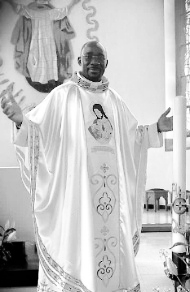
\includegraphics[scale=1.15]{../images/standing_daniel.png}
\end{wrapfigure}
Ainsi, la communion au Christ nous pousse à la communion fraternelle car l’Eucharistie est le pain de l’unité.
Tous nous pouvons y participer : à travers nos diversités, nous formons le corps du Christ. Notre source d’unité n’est pas le pays et la culture ; c’est le Christ qui nous invite à sa table. L'Eucharistie existe pour nous rapprocher les uns des autres, pour faire de nous un seul corps, le Corps du Christ. Il nous appartient d'en tirer les conséquences concrètes.



\begin{flushright}
Bonne méditation !
\textit{Père  Daniel  ETTÉ}
\end{flushright}


